% !TEX program = xelatex
% “华为杯”第二十三届中国研究生数学建模竞赛论文
% 模板：本目录 gmcmthesis.cls（按官方附件3 .doc 逐项实测复刻；规范见 docs/附件2）
% 编译：xelatex main && bibtex main && xelatex main && xelatex main
% 章节树冻结于 paper/outline.md v3（2026-09-25）：七章合并结构；
% 图表接线 = 正文正式 12 图 9 表，图号由 LaTeX 顺排（G1=图1），全部 \ref 引用。
\documentclass[colorprint]{gmcmthesis}

\baominghao{2026XXXXX}        % 参赛队号（提交前务必核对）
\schoolname{（学校名称）}
\membera{（队员一姓名）}
\memberb{（队员二姓名）}
\memberc{（队员三姓名）}
\title{复杂场景下多模态情感识别的数学建模与算法设计}

\begin{document}
\maketitle                    % 封面(页脚居中"0") + 摘要页页首(页码从 1 起，无页眉)

%% ============ 摘要页 ============
\begin{abstract}
（摘要正文：针对……问题，本文建立……模型。首先……；其次……；最后……。
主要结果与创新点：……。——最后写，素材见 draft/00-摘要.md）

\keywords{多模态情感识别；跨模态时序对齐；缺失鲁棒预测；可解释性}
\end{abstract}

%% ============ 目录（可选） ============
\maketoc

%% ============ 正文（章节结构冻结于 paper/outline.md v3） ============
\section{问题重述}
%（素材：题面 docs/复杂场景下多模态情感识别的数学建模与算法设计.docx）
% 1.1 背景 1.2-1.4 三问重述 1.5 附件说明（附件1 100 条原始；附件2 3395/728/727
% 特征；附件3 30 条缺失样本；附件4 20 条可解释专项）

\section{问题分析与总体技术路线}
%（素材：三重挑战→三问递进；接口约定与公共纪律）
2.3 节给出全文总体技术路线，如图~\ref{fig:g1}~所示：P1 建立统一语义—时间
坐标系，P2 在其上做缺失鲁棒预测，P3 利用 P1 映射表完成证据回溯，三问构成
闭环。
\begin{figure}[htbp]
  \centering
  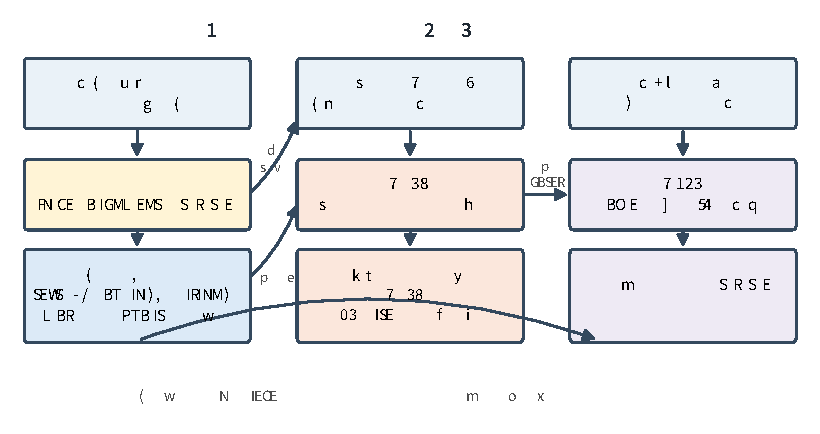
\includegraphics[width=\textwidth]{figures/g1_framework.pdf}
  \caption{全文总体技术路线：P1 统一表示 $\to$ P2 缺失鲁棒预测 $\to$ P3 反事实
  解释；底部旁路为 P1 映射表（WordPiece $\to$ 原词 $\to$ 物理时间）直供 P3 证据回溯。}
  \label{fig:g1}
\end{figure}

\section{模型假设与符号说明}
%（素材：3.1 假设 H1–H10 对齐 docs/实验假设与验证目标.md——含 H10 文本缺失
% 无泄漏；3.2 符号表 o/b/a、v(S)、φ、IG、g、α、S_select、D_S、T=1.2142）

\section{问题一：多模态时序对齐模型的建立与求解}
%（素材：docs/问题一建模方案.md v2.2；4.5 尾设"对题目要求点的回应"）
\subsection{统一语义—时间坐标系}
三问共用同一坐标系：WordPiece 位置域与音频/视觉物理时间域分离，仅以
词区间 $[t_s,t_e)$ 映射连接，见图~\ref{fig:q1-unified}。
\begin{figure}[htbp]
  \centering
  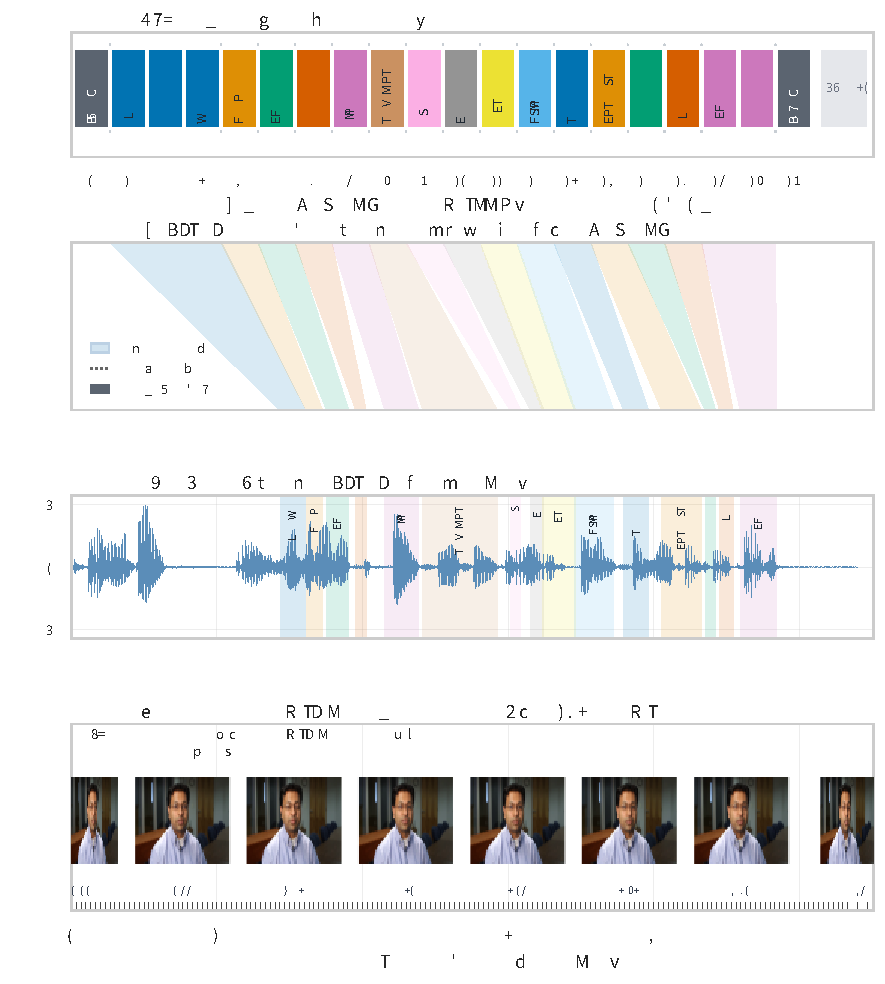
\includegraphics[width=\textwidth]{figures/q1/q1_unified_coordinate.pdf}
  \caption{统一语义—时间坐标图（样本 $-$3g5yACwYnA$_\$$13，VFR）：文本轨
  （position 域）、映射梯形带、音频波形轨与视觉关键帧轨（time 域，
  pts\_time 落位）；两域坐标独立，不做线性拉伸。}
  \label{fig:q1-unified}
\end{figure}

\subsection{50 步语义网格与状态掩码}
网格规则（多子词 $\alpha=1/n_{wp}$、标点继承、头部截断 CLS$+$48$+$SEP@49、
SEP 后无音视证据、词区间复制而非等间隔帧）见图~\ref{fig:q1-grid}。
\begin{figure}[htbp]
  \centering
  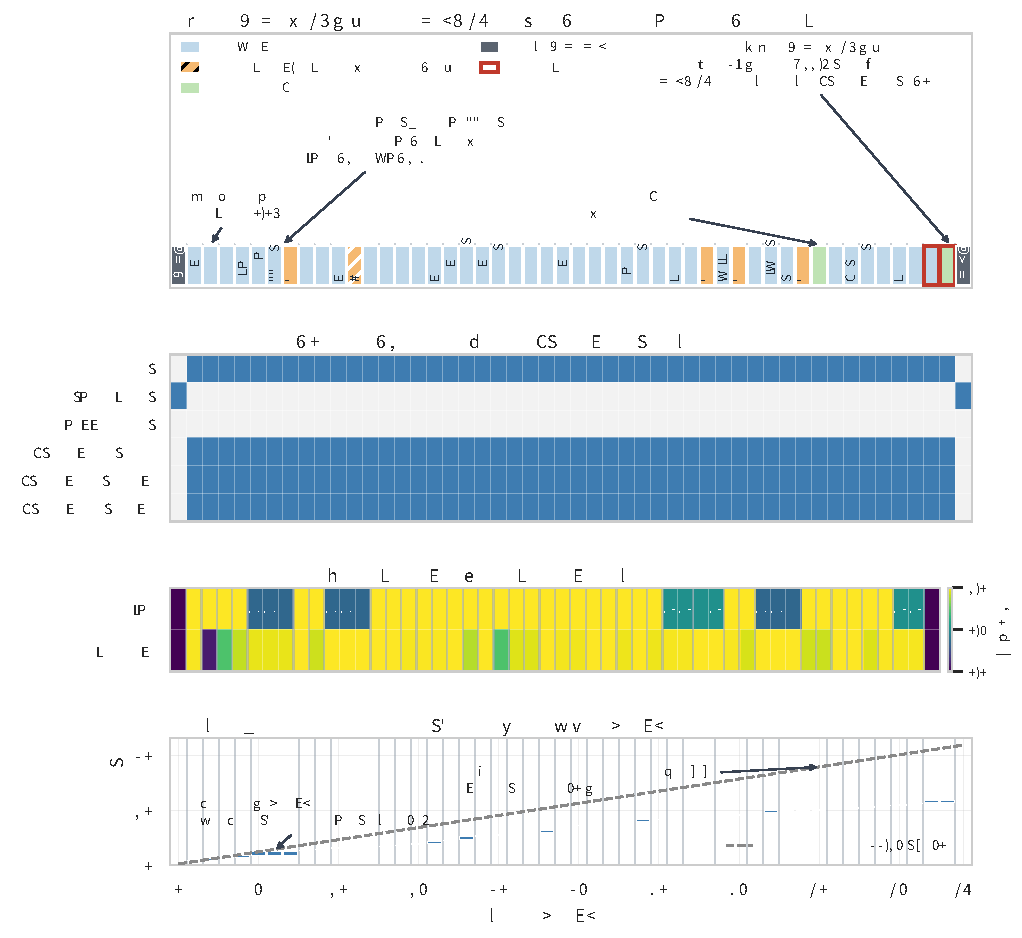
\includegraphics[width=\textwidth]{figures/q1/q1_semantic_grid.pdf}
  \caption{50 步语义网格与状态掩码（样本 $-$a55Q6RWvTA$_\$$3：65 词截断为
  39 词 $+$ 48 内容片；自冻结 pkl 自动生成）。}
  \label{fig:q1-grid}
\end{figure}

\subsection{对齐求解算法：CTC 强制对齐与失败分层处理}
%（插值放行 / 质量标记 / 人工核查清单；rollback 判定为数据异常样本随管线放行）

\subsection{四指标验收与对题面回应}
验收结果汇总于图~\ref{fig:q1-accept}~与表~\ref{tab:q1-acceptance}。
\begin{figure}[htbp]
  \centering
  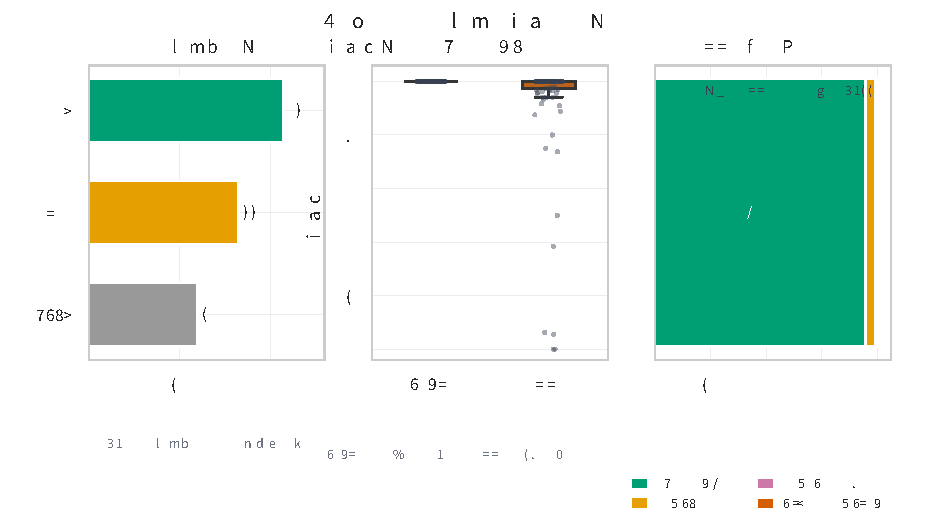
\includegraphics[width=\textwidth]{figures/q1/q1_acceptance_summary.pdf}
  \caption{P1 验收三联图：对齐质量状态分布（质量标记，非管线失败）、100 条
  观测率分布、vision 缺失原因构成（分母 = content 位置数 $N{=}2247$）。}
  \label{fig:q1-accept}
\end{figure}
\begin{table}[htbp]
  \centering\small
  \caption{问题一验收结果汇总}
  \label{tab:q1-acceptance}
  \begin{tabularx}{\linewidth}{@{}p{2.8cm}p{5.6cm}p{3.8cm}X@{}}
    \toprule
    验收项 & 实测值 & 参照基准 & 判定 \\
    \midrule
    覆盖完整性 & 100/100 一一对应，无缺失/重复/多余 & 附件1 label-100 & 通过 \\
    Schema 一致性 & 违例 0（shape/dtype/mask 分区/SEP 位） & p1.v2 契约 & 通过 \\
    BERT 留出一致性 & bitwise 7/7，cos$_{\min}$=1.000 & 附件2 test 重叠 7 条 & 通过 \\
    audio 非零率 & 1.00000 & 0.99915 & $|\Delta|$=0.085\,pp $\le$ 2\,pp \\
    vision 非零率 & 0.94704 & 0.94473 & $|\Delta|$=0.231\,pp $\le$ 2\,pp \\
    对齐质量状态 & ok/review/rollback = 43/33/24 & — & 质量标记，非管线失败 \\
    \bottomrule
  \end{tabularx}
  \par \smallskip
  \end{table}

\subsection{典型回放（自动回放）}
%（replay 图×9 进附录；签核完成前一律称"自动回放"）

\section{问题二：缺失场景下鲁棒情感预测模型的建立与求解}
%（素材：docs/问题二实施步骤.md §1–§9）
\subsection{缺失空间与 MRFN 架构}
缺失空间 $(M,P,R,L)$ 与 MRFN 数据流见图~\ref{fig:q2-arch}。
\begin{figure}[htbp]
  \centering
  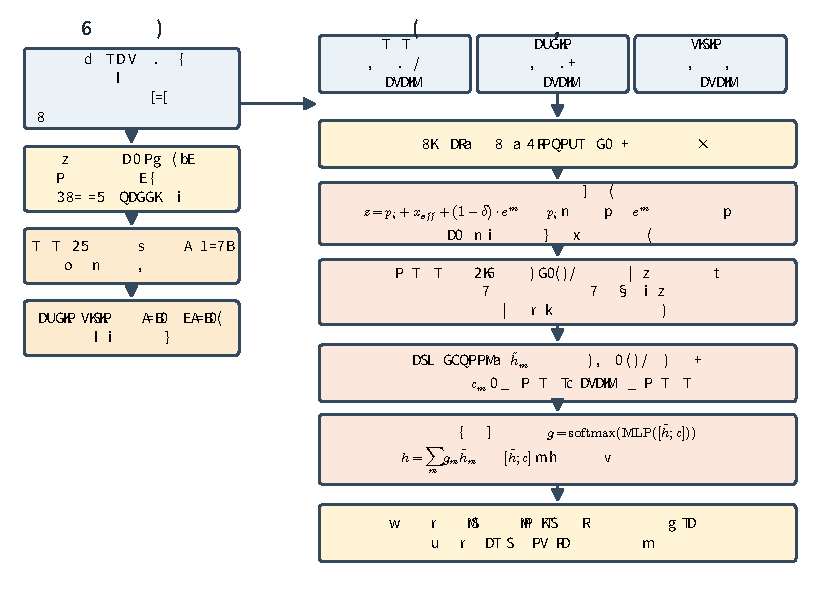
\includegraphics[width=\textwidth]{figures/q2/q2_mrfn_architecture.pdf}
  \caption{缺失空间与 MRFN 结构图（左列：$(M,P,R,L)$、$a{=}o\cdot(1{-}b)$、
  text 编码前 [MASK] 替换；右列：七层数据流，与代码契约逐条对应；
  输入维度为附件2 官方 74/35，区别于 P1 自产 25/23）。}
  \label{fig:q2-arch}
\end{figure}

\subsection{模型阶梯与 31 场景鲁棒性}
阶梯与退化结果见表~\ref{tab:p2-ladder}、图~\ref{fig:q2-deg}~与图~\ref{fig:q2-heat}。
\begin{table}[htbp]
  \centering
  \caption{模型阶梯评估结果}
  \label{tab:p2-ladder}
  \begin{tabularx}{\textwidth}{@{}lXrrrrrr@{}}
    \toprule
    模型 & 参数量 & Acc & macro-F1 & MAE & Pearson & $\mathcal{S}$ & $\overline{D_{\mathcal{S}}}$ \\
    \midrule
    B0 & 81,284 & 63.7\% & 60.0\% & 0.662 & 0.634 & 0.736 & 0.029 \\
    B1 & 93,764 & 65.7\% & 61.9\% & 0.644 & 0.653 & 0.749 & 0.035 \\
    B2 & 255,620 & 65.8\% & 61.0\% & 0.644 & 0.666 & 0.748 & 0.034 \\
    B3 & 429,380 & 65.0\% & 61.6\% & 0.631 & 0.665 & 0.748 & 0.035 \\
    MRFN & 416,839 & 66.7\% & 62.5\% & 0.634 & 0.675 & 0.756 & 0.028 \\
    \bottomrule
  \end{tabularx}
  \par \smallskip
  \end{table}
\begin{figure}[htbp]
  \centering
  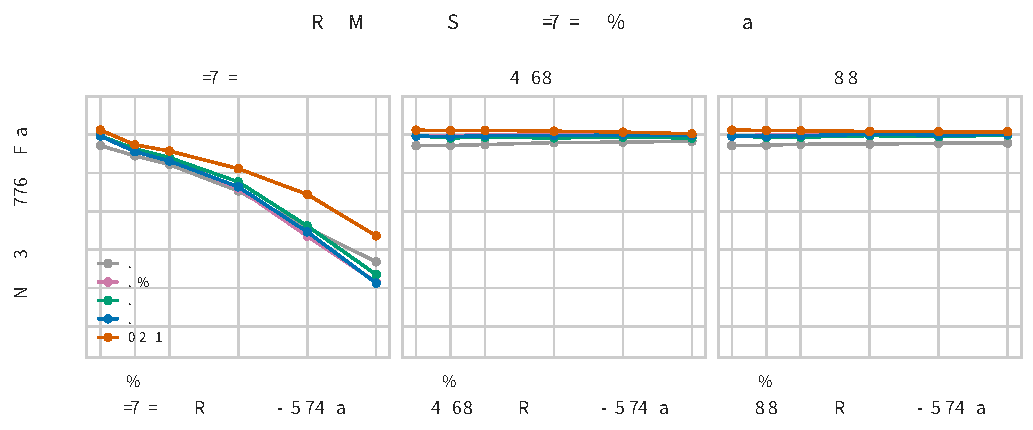
\includegraphics[width=\textwidth]{figures/q2/q2_degradation.pdf}
  \caption{缺失率—性能退化曲线（附件2 test，31 网格冻结协议）：MRFN 双优——
  clean $S{=}0.7561$ 最高且 text@80 退化最小（0.618 vs B3 0.557）。}
  \label{fig:q2-deg}
\end{figure}
\begin{figure}[htbp]
  \centering
  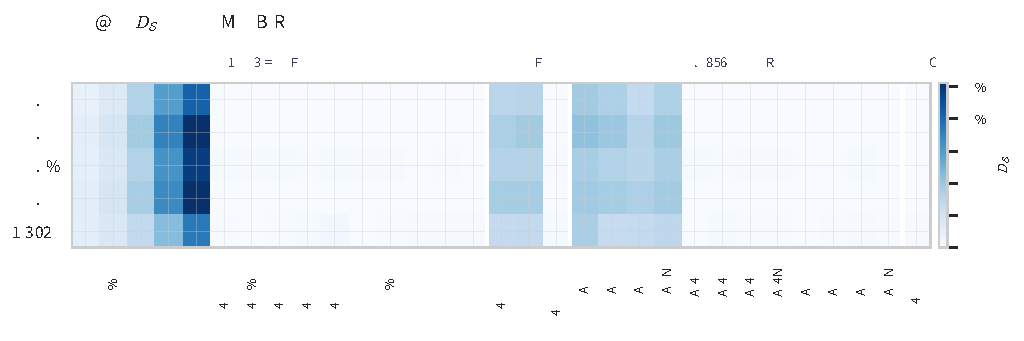
\includegraphics[width=\textwidth]{figures/q2/q2_scenario_heatmap.pdf}
  \caption{31 缺失场景性能退化热力图（$D_S$，颜色越深退化越大）。}
  \label{fig:q2-heat}
\end{figure}

\subsection{迁移与消融}
见 2$\times$2 迁移表（表~\ref{tab:p2-transfer}）与消融表（表~\ref{tab:p2-ablation}）。
\begin{table}[htbp]
  \centering
  \caption{2$\times$2 迁移表（同架构只变训练方式，$\mathcal{S}$）}
  \label{tab:p2-transfer}
  \begin{tabular}{lcc}
    \toprule
    训练方式$\backslash$测试 & clean test & 31 场景均值 \\
    \midrule
    clean 训练 & 0.736 & 0.705 \\
    缺失增强训练 & 0.756 & 0.735 \\
    \bottomrule
  \end{tabular}
  \par \smallskip
  {\small 注：$\mathcal{S}$ 为综合效用分；clean test 为附件2 测试集 clean 子集；31 场景均值为评测网格的等权平均（先场景内 8 实例、后 31 场景）。}
\end{table}
\begin{table}[htbp]
  \centering
  \caption{消融与填充基线（$S$，3-seed 均值；$\Delta$ 相对完整 MRFN 的 31 场景均值，自动生成）}
  \label{tab:p2-ablation}
  \begin{tabular}{lrccc}
    \toprule
    变体 & 参数量 & clean $S$ & 31 场景均值 $S$ & $\Delta$ \\
    \midrule
    MRFN（完整） & 416,839 & 0.756 & 0.735 & — \\
    去除缺失状态编码 & 413,447 & 0.739 & 0.723 & -0.012 \\
    去除掩码注意力 & 416,839 & 0.741 & 0.719 & -0.015 \\
    去除门控 & 432,772 & 0.733 & 0.718 & -0.017 \\
    去除缺失增强训练 & 416,839 & 0.736 & 0.705 & -0.030 \\
    B3 + zero 填充基线 & 429,380 & 0.737 & 0.716 & -0.019 \\
    B3 + 前向填充基线 & 429,380 & 0.736 & 0.714 & -0.021 \\
    \bottomrule
  \end{tabular}
\end{table}

\subsection{模型改进、采纳与追加终评}
MRFN 为附件2 主表的冻结正式模型；MRFN+ 为 valid 预注册筛选后采纳的补充
变体，其追加 test 结果不替换主表、亦无 31 场景鲁棒性曲线（表~\ref{tab:p2-final}，
评估批次列区分两种口径）。
\begin{table}[htbp]
  \centering
\caption{最终测试集结果（附件2 test，clean 口径）}
  \label{tab:p2-final}
  \begin{tabular}{llrrrr}
    \toprule
    模型 & 评估批次 & Acc & macro-F1 & MAE & $\mathcal{S}$ \\
    \midrule
    MRFN & 主表首次 test & 66.71\% & 62.52\% & 0.634 & 0.756 \\
    MRFN+（单模型均值） & 预注册追加 test & 67.45\% & 62.80\% & 0.644 & 0.760 \\
    MRFN+（3-seed 集成） & 预注册追加 test & 68.64\% & 63.86\% & 0.614 & 0.769 \\
    \bottomrule
  \end{tabular}
  \par \smallskip
  {\small 注：MRFN 为主表冻结正式模型；MRFN+ 为预注册追加评估的补充变体，未做 31 场景评估、不构造鲁棒性曲线；单模型均值与三种子集成为不同口径，不可直接比较。}
\end{table}

\subsection{附件3 交付（无标签，仅行为分析）}
行为分析见图~\ref{fig:q2-fj3}：门控与 text-only 一致率两组均未观察到预期的
单调重分配/趋同，如实报告。
\begin{figure}[htbp]
  \centering
  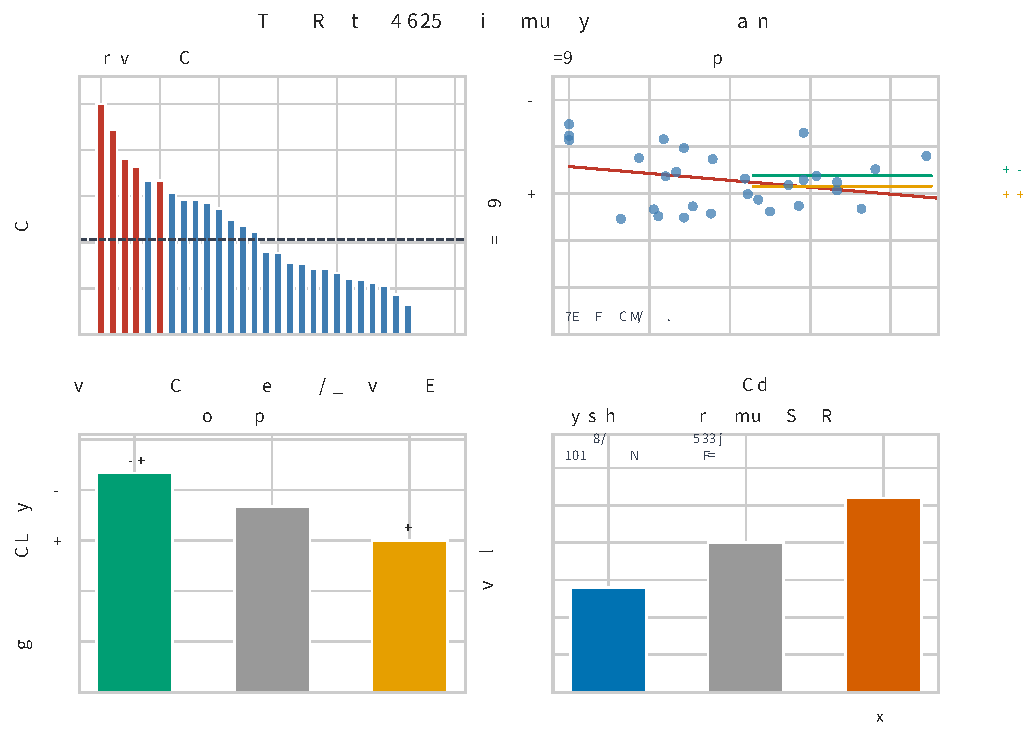
\includegraphics[width=\textwidth]{figures/q2/q2_fj3_behavior.pdf}
  \caption{附件3 行为分析（MRFN+ 集成，30 条，无标签不做精度声明）：joint
  缺失率、$g_{text}$ 与 a/v 缺失、text-only 一致率、预测极性分布。}
  \label{fig:q2-fj3}
\end{figure}

\section{问题三：可解释情感预测模型的建立与求解}
%（素材：paper/draft/06-问题三.md 成稿 + docs/问题三实施步骤.md）
\subsection{任务与两参照系}
Shapley 用联盟级 $v(\emptyset)$（avail$\equiv$0）；IG 用条件特征基线
（avail 固定自然观测 $o$），二者严格分名，见图~\ref{fig:q3-shapley}。
\begin{figure}[htbp]
  \centering
  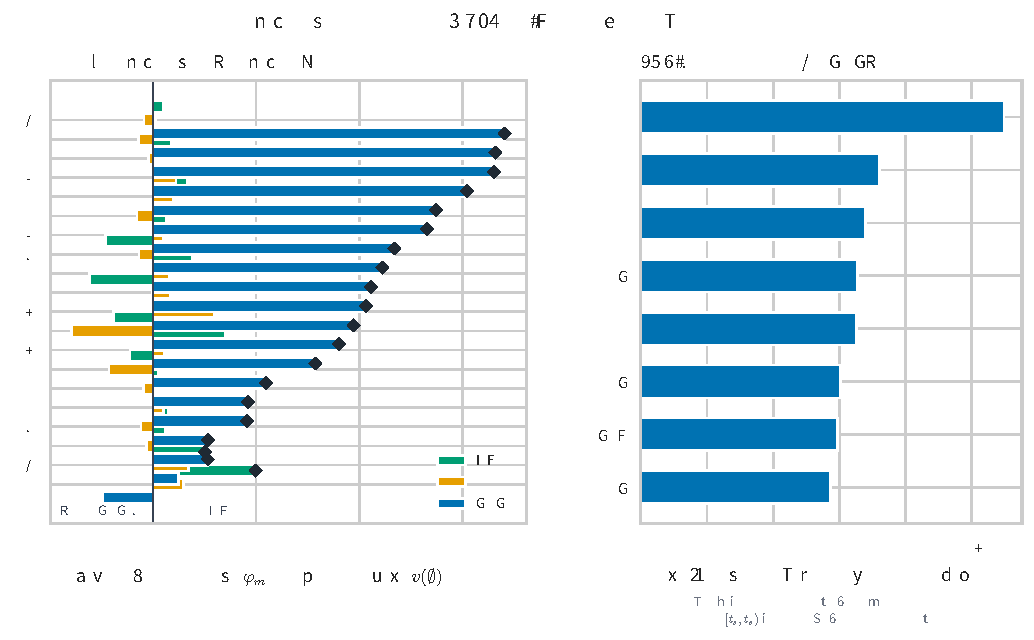
\includegraphics[width=\textwidth]{figures/q3/q3_shapley_evidence.pdf}
  \caption{模态贡献—证据回溯（附件4，20 条）：左为带符号 Shapley 贡献
  $\varphi_m$ 与主导模态（text 18 / vision 2），右为 TOP-8 原词证据
  （IG，条件特征基线）；附件4 无时间戳，词回溯用 P1 网格（20/20 对齐），
  $[t_s,t_e)$ 时间回溯仅 P1 域内可用。}
  \label{fig:q3-shapley}
\end{figure}

\subsection{Shapley 联盟归因}
完备性与方向统计见表~\ref{tab:p3-direction}、表~\ref{tab:p3-completeness}。
\begin{table}[htbp]
  \centering
\caption{模态 Shapley 方向表（预测类上带符号 $\varphi$；$v(\emptyset)$ 联盟级基准）}
  \label{tab:p3-direction}
  \begin{tabular}{lccc}
    \toprule
    模态 & $\varphi{>}0$ & $\varphi{<}0$ & 主导 \\
    \midrule
    text & 19 & 1 & 18 \\
    audio & 10 & 10 & 0 \\
    vision & 13 & 7 & 2 \\
    \bottomrule
  \end{tabular}
\end{table}
\begin{table}[htbp]
  \centering
\caption{Shapley 完备性（$\sum_m \varphi_m = v(N)-v(\emptyset)$，逐样本）}
  \label{tab:p3-completeness}
  \begin{tabular}{lccc}
    \toprule
    输出头 & 最大残差 & 门槛 & 通过 \\
    \midrule
    分类 & $3.0\times10^{-8}$ & $1{\times}10^{-5}$ & 20/20 \\
    强度 & $4.4\times10^{-16}$ & $1{\times}10^{-5}$ & 20/20 \\
    \bottomrule
  \end{tabular}
\end{table}

\subsection{积分梯度位置归因}
64 步中点积分逐样本 40/40 通过（max 相对误差 0.62\%），结构位泄漏为零，
验证见图~\ref{fig:q3-igval}~与表~\ref{tab:p3-ig-validation}。
\begin{table}[htbp]
  \centering\small
\caption{IG 验证结果}
  \label{tab:p3-ig-validation}
  \begin{tabular}{p{2.9cm}p{3.3cm}p{3.6cm}l}
    \toprule
    验证项 & 实测 & 门槛/口径 & 判定 \\
    \midrule
    积分误差（64 步中点） & 40/40 & max rel 0.62\% & 通过 \\
    阻断位泄漏 & max $|IG|$=0（逐位精确） & 3基线$\times$2输出$\times$3模态 & 通过 \\
    \#13 哑玩家 & $\max|IG_v|$=0（逐位精确） & $\varphi_v\equiv 0$ & 通过 \\
    问题一网格映射 & 20/20 & 截断词 22 个未覆盖 & 通过 \\
    基线排序敏感性 & $\bar\rho_{min}$=0.961 & $\ge 0.96$ & 通过 \\
    稳定性 t/a/v & 0.997/0.995/0.984 & text $\ge 0.6$ & 通过 \\
    \bottomrule
  \end{tabular}
\end{table}
\begin{figure}[htbp]
  \centering
  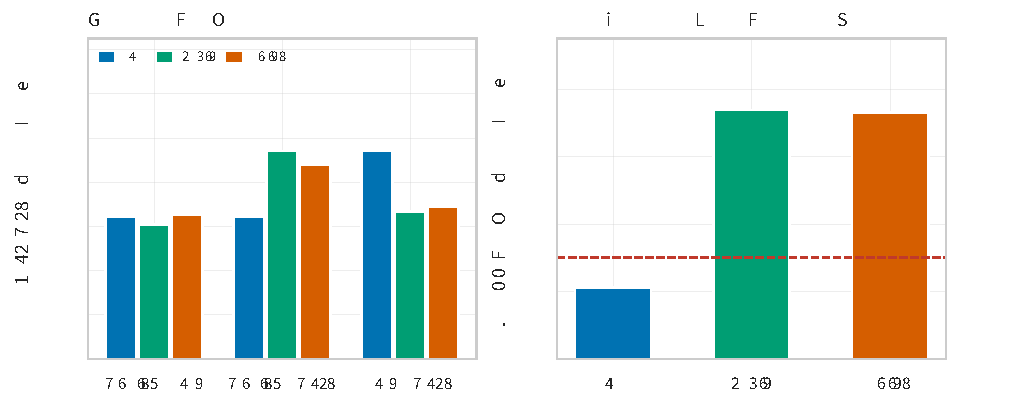
\includegraphics[width=\textwidth]{figures/q3/q3_ig_validation.pdf}
  \caption{IG 验证：三基线排序高度一致（$\bar\rho\ge 0.96$）；F 诊断——
  a/v 局部干预下 IG--LOO 强一致，text 未达门槛。}
  \label{fig:q3-igval}
\end{figure}

\subsection{解释可信性验证：A--E 通过与 F 项结构性诊断}
删除/插入保真度曲线见图~\ref{fig:q3-fid}，六门槛验收见表~\ref{tab:p3-fidelity}：
A--E 通过（A 删除逐样本胜 19/20），F 项 text IG--LOO 0.170 未达 0.3 门槛，
已完成结构性诊断（text [MASK] 重编码为非局部干预，与嵌入层 IG 属不同反事实）。
\begin{figure}[htbp]
  \centering
  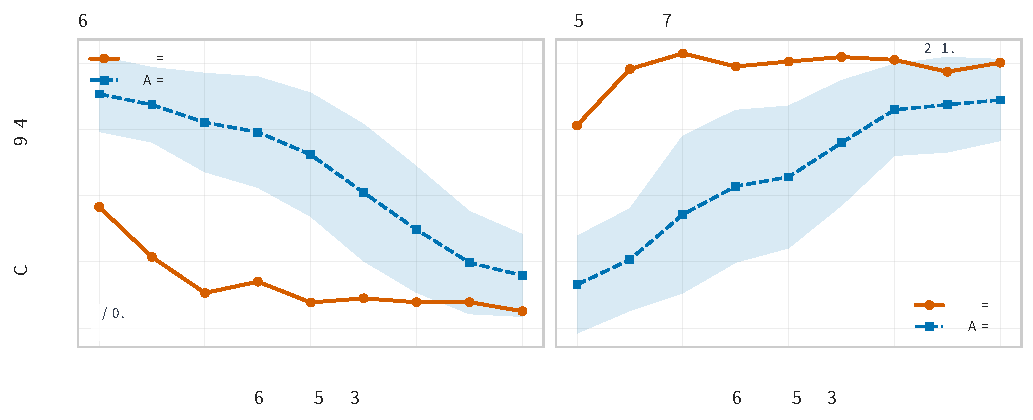
\includegraphics[width=\textwidth]{figures/q3/q3_fidelity.pdf}
  \caption{删除/插入保真度曲线（M3 主基线 IG$_{cls}$）：归因排序显著优于
  随机排序（AOPC $=0.1657$，胜 19/20；$\Delta$AUC $=0.1291$，胜 20/20）。}
  \label{fig:q3-fid}
\end{figure}
\begin{table}[htbp]
  \centering\small
\caption{解释保真度六项检验结果}
  \label{tab:p3-fidelity}
  \begin{tabularx}{\linewidth}{@{}p{2.2cm}p{5.2cm}p{3.9cm}X@{}}
    \toprule
    门槛 & 实测 & 预注册规则 & 判定 \\
    \midrule
    A 删除 & 0.166（胜 19/20） & 均值$>$0 且 $\ge$15/20 & 通过 \\
    B 插入 & 0.129（胜 20/20） & 均值$>$0 且 $\ge$15/20 & 通过 \\
    C 全面/充分 & compr=0.306，|suff|=0.098 & compr$>$0，$|$suff$|<$compr & 通过 \\
    D 随机化坍缩 & median $\rho$ max 0.267 & $\le 0.3$ & 通过 \\
    E 稳定性（text） & 0.997 & $\ge 0.6$ & 通过 \\
    F text IG--LOO & 0.170 & $\ge 0.3$ & \textbf{未通过} \\
    \bottomrule
  \end{tabularx}
  \par \smallskip
  \end{table}

\subsection{g--$\varphi$ 关系}
%（素材：valid 728 点 g–φ 散点，text Spearman 0.716；a/v 较弱如实写）

\subsection{附件4 交付与解释卡}
解释卡（无标签，不做精度声明，仅展示预测/贡献/证据回溯）见
图~\ref{fig:q3-cards}：\#09（强 text 主导）、\#14（唯一 vision 主导）、
\#13（vision 全模态自然缺失的哑玩家，$\varphi_v\equiv 0$）。
\begin{figure}[htbp]
  \centering
  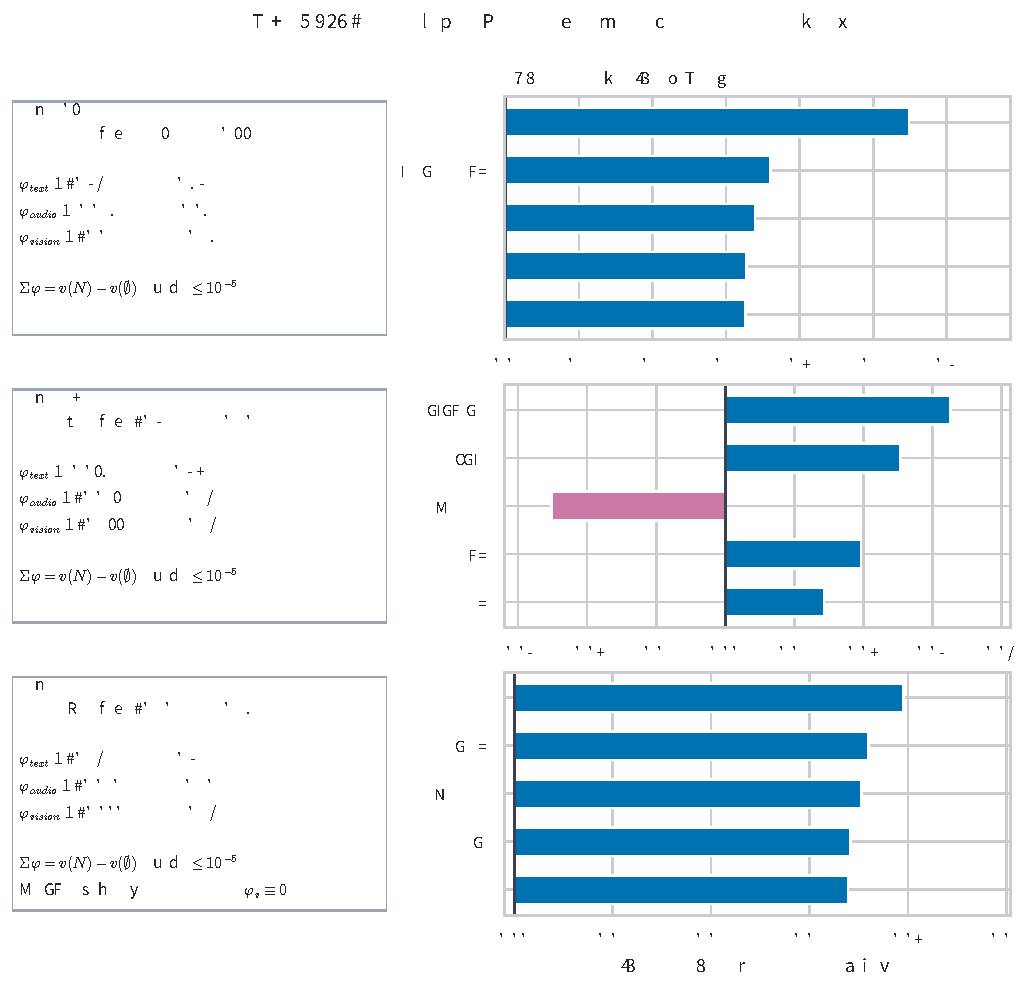
\includegraphics[width=\textwidth]{figures/q3/q3_explain_cards.pdf}
  \caption{解释卡三例（附件4，MRFN+ 3-seed 集成）：左列预测与模态贡献，
  右列 TOP-5 原词证据（词聚合 = P1 $\alpha$ 映射 + 质量守恒求和）。}
  \label{fig:q3-cards}
\end{figure}

\subsection{局限}
%（P3 四条局限，draft/06 已成稿）

\section{模型综合评价与推广}
%（原"实验与结果分析+模型评价与推广"合并；只做跨问题综合分析，不重复分问指标）
\subsection{优点}
%（契约化管线 / 预注册纪律 / 缺失感知闭环）
\subsection{三问联合验证：门控—信息量—贡献关系及其边界}
%（不写"三角互证"：a/v g–φ 较弱 + text IG–LOO 反事实语义差异，边界如实写）
\subsection{局限与错误归因}
%（P3 四条 + P2 弱带与帕累托 + P1 回放签核待办；同文本跨标签不可约误差）
\subsection{推广}
%（流式、跨域多模态、医学时序）

%% ============ 参考文献 ============
\bibliographystyle{gmcm}
\bibliography{reference}

%% ============ 附录 ============
\appendix
\section{环境与核心参数}
%（素材：docs/环境与复现说明.md、environment-manifest.json 字段表）

\section{关键代码}
\begin{Python}{align.py（示例：P1 词区间对齐）}
# TODO: 从 src/ 摘取关键片段
\end{Python}

\section{P1 自动回放图}
%（replay_×9；签核完成前一律称"自动回放"；q1 旧图与 q3 备选图亦可放此）

\end{document}
